\setcounter{page}{1}% Start page number with 1
\belowdisplayshortskip=0pt
\renewcommand{\thepage}{\arabic{page}}% Arabic numerals for page counter
\chapter{Introduction}

Traditionally, dark matter has been simulated by using N-body schemes, in which the temporal evolution of a system of N particles is simulated usually by solving the Poisson-Vlasov equation \cite{2012PDU150K}.
These N-body simulations have been essential for the development of modern cosmology and the characterization of dark matter halos.
For example, the development of the $\Lambda$CMD cosmology was heavily linked with a classic N-body simulation of the large scale structure of the universe which used only 32748 particles! \cite{1985ApJ292371D}.

On the other hand, Lattice-Boltzmann simulations have been widely used to recreate increasingly complex fluids and boundary conditions, nonetheless, the usual Lattice-Boltzmann scheme does not simulate the entire velocity space, but simply a small number of adventive velocities. 

Inspired by the work of Philip Mocz, Sauro Succi \cite{integerLatticeDynamics}, and Sebastian Franco \cite{franco}, in which a Lattice-Boltzmann simulation is used to simulate the phase space of a \emph{collisionless} one dimensional dark matter fluid. We implement a Lattice-Boltzmann simulation of the phase space of a \emph{collisional} three dimensional dark matter fluid using the BGK approximation for the collisional term.

\section{General objetive}
To simulate the phase space of a collisional dark matter fluid using a Lattice-Boltzmann method.
\section{Specific objetives}
\begin{itemize}
\item To implement a Lattice-Boltzmann simulation using a 2-dimensional phase space and a varying collisional term.
\item To implement a Lattice-Boltzmann simulation using a 4-dimensional phase space and a varying collisional term.
\item To implement a Lattice-Boltzmann simulation using a 6-dimensional phase space and a varying collisional term.
\item To simulate the phase space of a collisional dark matter fluid using literature values for the thermally averaged cross-section and compare it with its collisionless version.
\end{itemize}


\newpage
In order to follow the ideas and developments of the upcoming chapters, it is essential to understand some concepts and computational techniques.
In this chapter, we present all the necessary knowledge for the proper understanding of this work.

\section{Dark Matter}
Modern cosmology describes the universe as being composed of two fundamental types of energy: dark energy and matter\footnote{In relativity, mass and energy are equivalent.}, with dark energy being associate with a cosmological constant and matter being divided into two categories: dark matter and standard model matter\footnote{Which often is called \tqt{Baryonic matter} due to Baryons being the largest fraction of this mass.}.
The energy density of the universe is $69\%$ dark energy and $31\%$ matter\cite{2018arXiv180706209P}.


Standard model matter includes all the particles whose interactions can be properly described by the standard model, such as: Protons, Electrons, Atoms and naturally, any structure that they form, like humans or stars.
On the other hand, dark matter is all the matter we measure from astrophysical sources which cannot be explained by baryonic matter.
We know of the existence of dark matter entirely from astrophysical evidence, during this section we are going to do an historical review of such evidence.

\subsection{The Cluster Missing Mass Problem}
The traditional history of dark matter begins in the 1930s with the swiss astronomer Fritz Zwicky\cite{aHistory} \cite{tasiCline}, who noticed an unusually high velocity dispersion between the galaxies of the Coma Cluster.
To tackle the problem, Zwicky assumed that the Coma Cluster \tqt{had already reached a mechanically stationary state} \cite{englishZwicky} and such, the virial theorem could be applied.
By counting galaxies, along with assuming that matter is distributed uniformly in the cluster and using Hubble's estimate of the mean mass of a galaxy, Zwicky was able to estimate the potential energy of the Cluster.
Using his estimate of the visible mass and the virial theorem, Zwicky concluded that the velocity dispersion must be $\sqrt{\bar{v^2}} = 80$ km/s.
Nonetheless, the real measurement of the velocity dispersion was $\sqrt{\bar{v^2}} = 1000$ km/s, implying a virial mass about 400 times larger than the visible mass\footnote{This ratio is often called the mass-to-light ratio.}.
Zwicky called the discrepancy between the luminous matter (in the form of visible galaxies which could simply be counted) and the virial matter (obtained from the virial theorem and the high velocity dispersion of the cluster) \tqt{Dark Matter}.

By the late 1950s similar calculations for different clusters had been published. Many of those calculations had very large values for the mass-to-light ratio\cite{schwarzschildSon}, which were consistent with the mass-to-light ratio calculated from the Coma Cluster. The problem of the missing mass seemed to appear in almost every large scale structure in the universe, and by the early 1970s astrophysicist had already disregarded hot gas\cite{meekins} and free hydrogen\cite{penzias} as explanations for the missing mass in Clusters.
Nonetheless, it was still possible that the missing mass problem could be in fact solved by a more refined model of the cluster kinematics, because so far, the missing mass problem had only been observed on Clusters and large scale structures.

\subsection{Galaxy Rotation Curves}
A galaxy rotation curve plots the orbital velocity of stars in a galaxy versus their distance to the galaxy centre.
These curves became very informative thanks to the work of the Indian astrophysics Subrahmanyan Chandrasekhar, who proved that the mutual interactions between stars were negligible, so a galaxy could be modeled as a non-interacting system of stars \cite{chandrasekhar}. Such modeling allows to obtain mass profiles from galaxy rotation curves.
Now, due to photometric measurements, astrophysicist believed that most of  galaxy's mass was overwhelmingly concentrated in the galaxy centre, therefore, it was reasonable to model the galaxy similarly to the solar system.

Consider a star in the galaxy disk with mass $m$ at a distance $r$ from the galaxy centre.
Given that we can disregard the interaction between starts, the sum of forces acting on the object is simply the gravitational attraction towards the galaxy centre:
\begin{equation}
\label{heh}
m\frac{v^2}{r} = G \frac{mM}{r^2}
\end{equation}\\
\vspace{-1mm}With $M$ being the mass enclosed by the star orbit and $v$ being the orbital velocity of the star. Finally, the galaxy rotation curve for such galaxy will be given by:
\begin{equation}
v(r) = \sqrt{\frac{GM}{r}}
\end{equation}%\vspace{2mm}
Which means that for objects outside of the galaxy disk (but still under the influence of the galaxy gravitational pull) the enclosed mass will be constant regardless of the radius, and thus, the orbital velocity will be proportional to $r^{-1/2}$. With the advent of radio astronomy and the invention of the Image Tube Spectrograph, astronomers were able to measure orbital velocities way beyond the apparent end of the luminous galaxy disks, only to find that the orbital velocity did not decay proportionally to $r^{-1/2}$ but it stayed more or less constant\cite{h21Line} \cite{galactoDistance} \cite{veraFirst}. This behavior can be seen easily in the figure \ref{galaxyCurve}:%\cite{parnovskyCosmology} TODO
\begin{figure}[ht]
    \centering
    %\includegraphics[width=10cm,height =7cm]{Diapositiva1.jpg}
    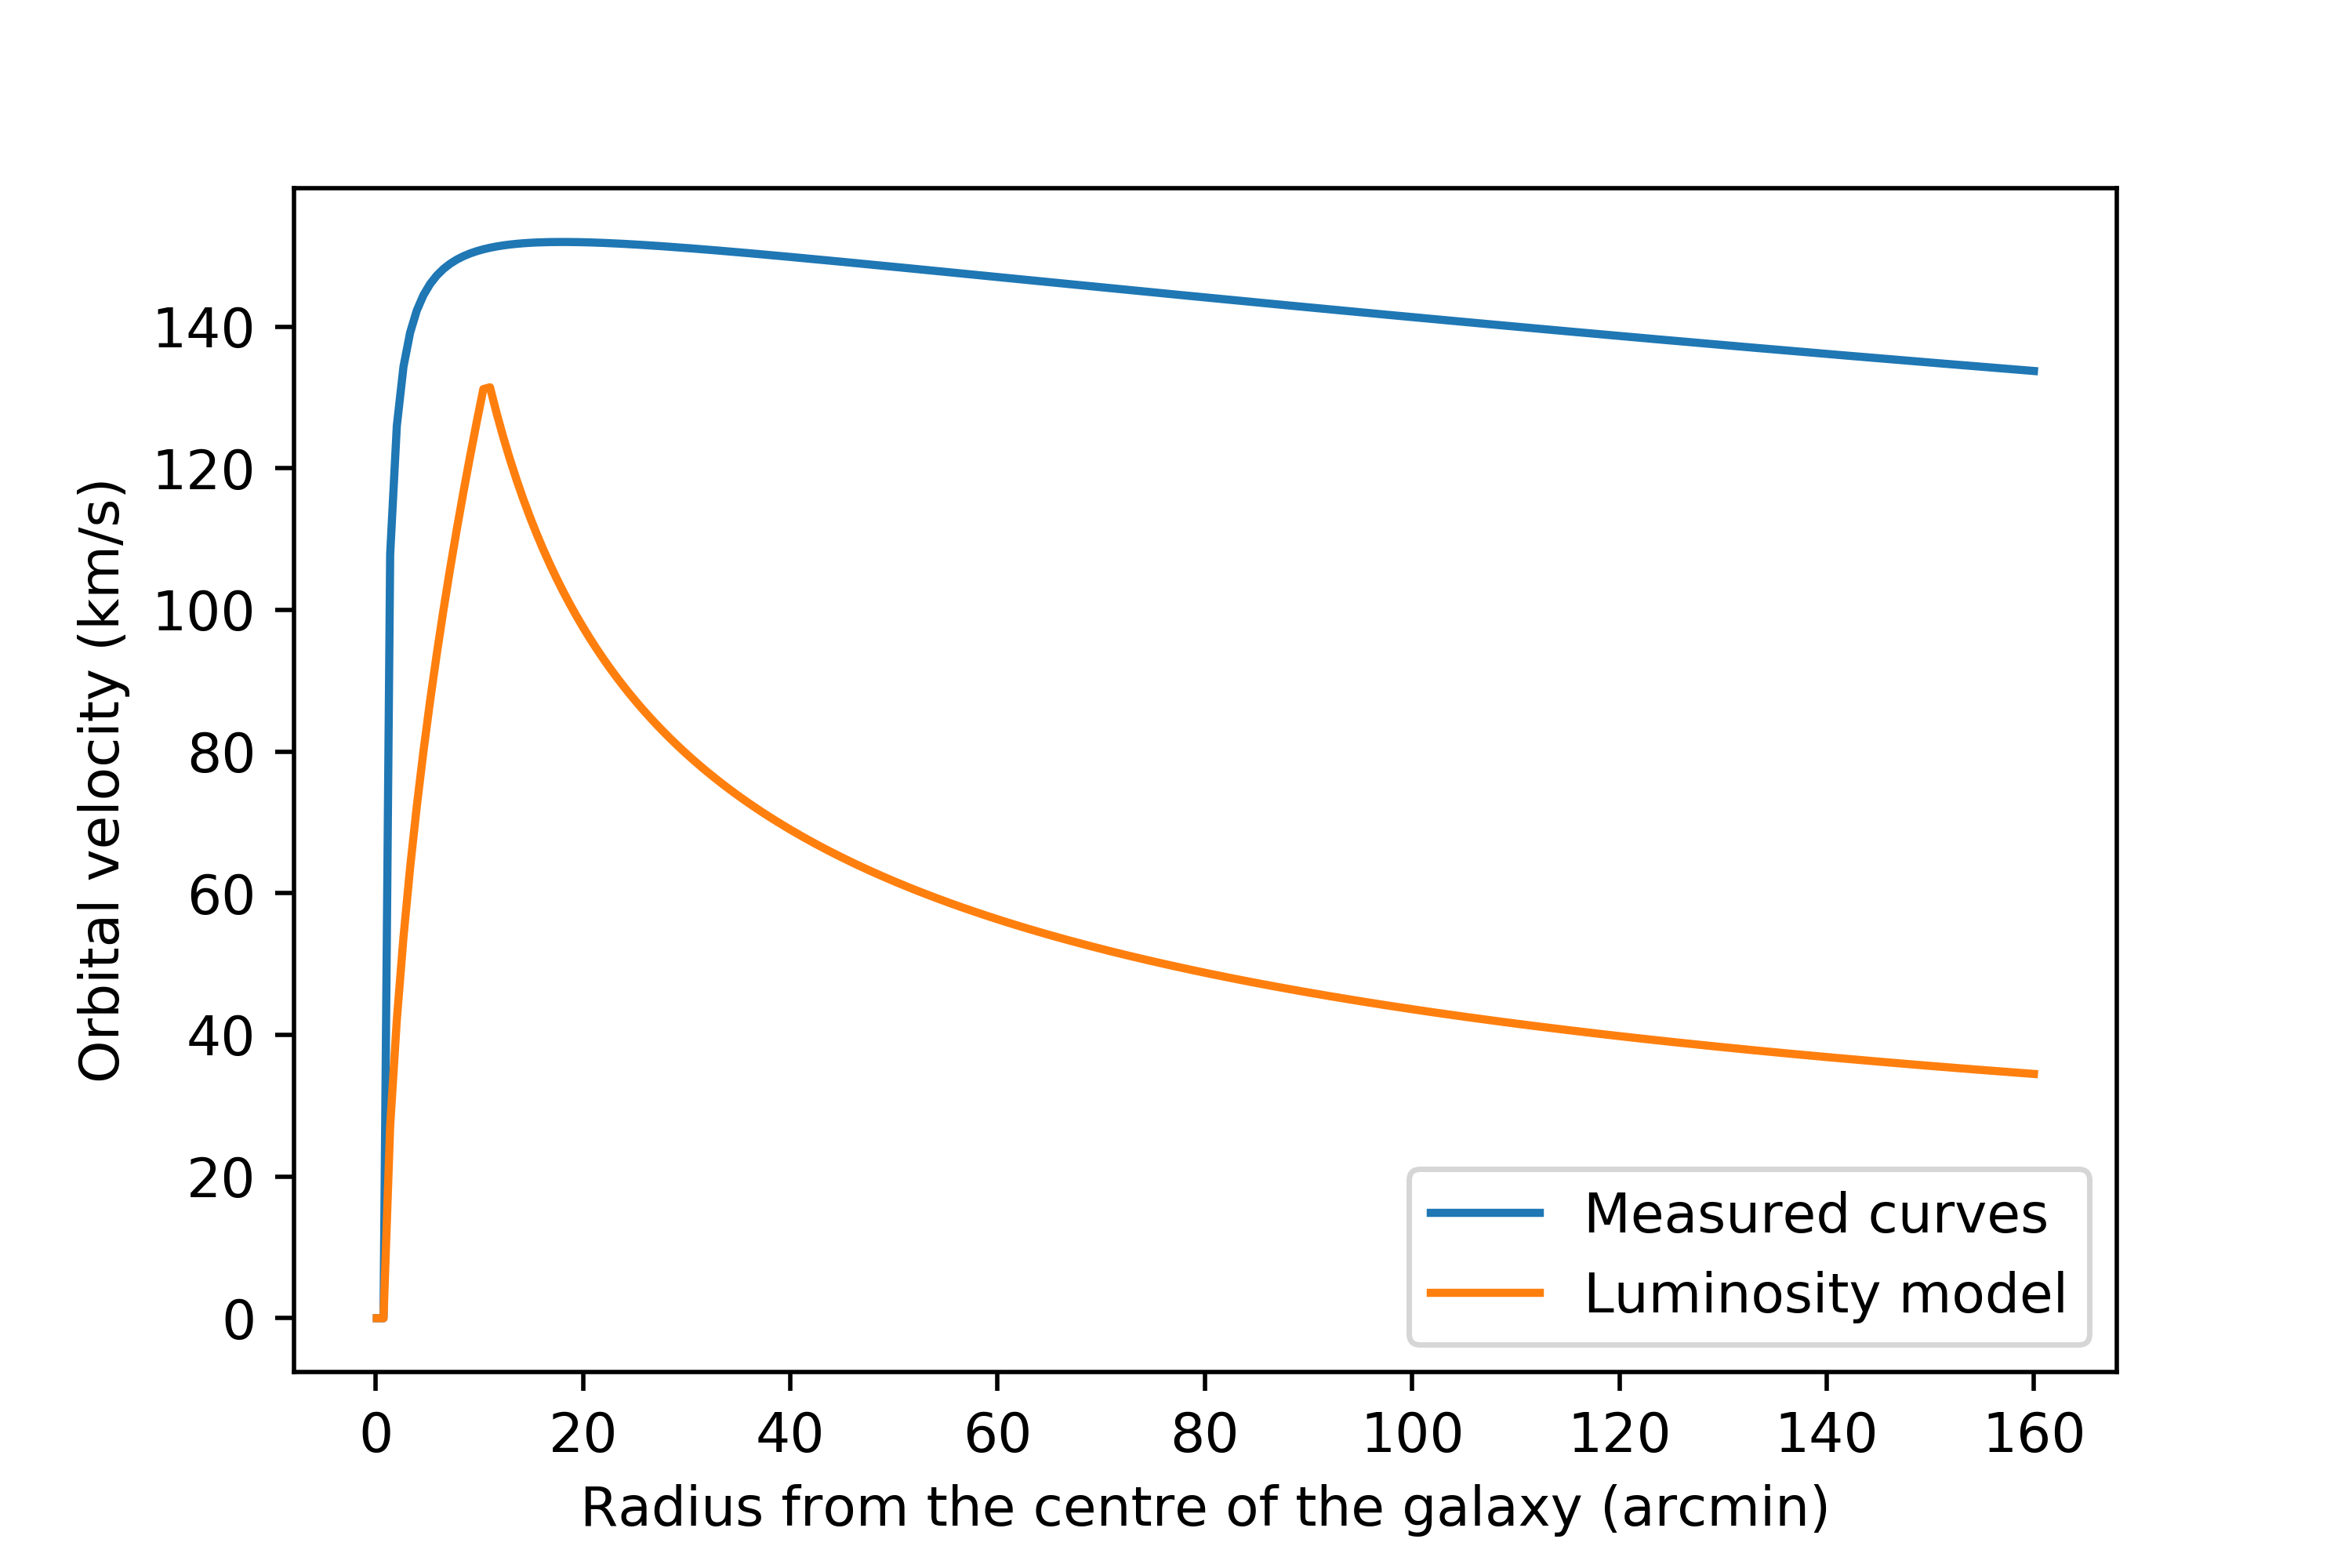
\includegraphics[scale=0.8]{imag/galaxyRotCurv.png}
    \caption{A comparison between the model from photometrical measurements and the curves measured. This curves are illustrative and do not correspond to a particular galaxy.}
    \label{galaxyCurve}
\end{figure}

This unexpected velocity profile implied a mass-to-light ratio that increased with distance and also the existence of mass beyond the visible galactic disk\cite{theIsMassOutside}.
The overwhelming amount of high quality galaxy rotation curves measurements, let to the acceptance of the dark matter hypothesis in the astrophysical community.

Throughout the use of numerical simulations and the measurement of more galaxy rotation curves during the 1980s and the 1990s, it was concluded that the dark matter density in galaxies was well modeled by the Navarro-Frenk-White (NFW) profile\cite{FWN}\cite{mariangela}
\begin{equation}
\rho(r) = \frac{\rho_0}{r/r_s(1+r/r_s)^2}
\end{equation}
\subsection{The Bullet Cluster}
\label{bulletExplain}
Galaxy clusters have three main constituents: dark matter, intracluster gas (which is mostly ionised hydrogen and helium), and the galaxy themselves.\cite{book:75345}

We can observe the intracluster baryonic matter in the x-ray band thanks to Bremsstrahlung radiation, therefore, by doing photometry in X-ray it is possible to map the baryonic gas distribution in a cluster.
In the case of dark matter, we infer its existence in clusters thanks to the work of Fritz Zwicky and the posterior work in the missing mass problem in galaxy clusters.
Our current estimates place most of the cluster mass in the dark matter component.
By analyzing the gravitational lensing effect (in particular the \emph{weak} gravitational lensing effect) it is possible to map the mass distribution of a galaxy cluster. 
Lastly, we can observe the galaxies in the visual and the infrared band.
They are the only component of a galaxy cluster that can be observed in the visual band.
About 90 percent of the mass of a cluster is dark matter (this is not a surprise since Fritz Zwicky measured mass-to-light ratios of 50 during the 1930s). Of the remaining baryonic matter, the ionized gas mass can represent up to 90$\%$ of the mass, making galaxies responsible of about 1$\%$ of the total cluster mass.

The object Bullet Cluster (also known as 1E 0657-558) is the aftermath of the collision of two galaxy cluster.
Before the collision, each cluster had its own set galaxies, baryonic gas and dark matter, and the centroid of each constituent coincided with the center of mass of the whole cluster.
During the collision, each constituent reacts differently to the situation:
\begin{itemize}
\item Galaxies, given that they occupy a minuscule fraction of the total volume of the cluster, are essentially collisionless. Two galaxy clusters can collide without any galaxy (or very little galaxies) colliding per se. 
\item Dark matter is also modeled as collisionless, therefore, during the collision of two galaxy clusters, the dark matter components simply pass through, similarly to how Neutrinos constantly cross the Earth without losing a significant amount of energy.
\item The baryonic gas on the other hand is collisional, and its short range interactions are very well described by the Standard Particle Model. During the galaxy cluster collision, the baryonic parts interact and they lose energy through particle collision. This interaction decouples the baryonic gas from the galaxies and dark matter, and, given that we can directly observe the hot gas (thanks to X-ray astronomy), we can measure the separation between the centroid of the hot gas and the centroid of the galaxies.
\end{itemize}

If there was no dark matter, then after the collision the weak lensing mapping of the mass distribution would be very close to the hot gas distribution, because the hot gas would be the dominant mass density in the cluster. If dark matter were to exists, then it would dominate the mass density distribution in the galaxy cluster and the weak lensing mapping would be very similar to the galaxies distribution (because they are also collisionless).

What we observe in the Bullet Cluster is the latter case, in which hot gas decouples from dark matter and galaxies.
By mapping the cluster components and measuring the difference between the centroids, it was concluded that there is a dark matter component in the clusters.
Very accurate measurements and estimates of the centroids show a small collisional nature in the dark matter component, such measurements allows estimate the \emph{thermally averaged cross-section} of the dark matter particle ($<\sigma v>$).
Therefore, it is worth exploring the collisional dark matter scenario.

\section{The Boltzmann Equation}
The Boltzmann equation was originally proposed in 1872 by Ludwig Boltzmann and is used to model the behavior of statistical systems outside of the equilibrium. 
Formally, the Boltzmann equation describes the evolution of the phase space of a typical dark matter particle, such that $\f \dd \vb{r} \dd \vb{v}$ is the probability of finding the dark matter particle in a position between $\vb{r}$ and $\vb{r} + \dd \vb{r}$, with velocity velocity between $\vb{v}$ and $\vb{v} + \dd \vb{v}$.
Given than a halo is made of typical dark matter particles, we can treat it as a dark matter fluid and apply the Boltzmann equation now interpreting $\f \dd \vb{r} \dd \vb{v}$ as the number of dark matter particles whose position is between $\vb{r}$ and $\vb{r} + \dd \vb{r}$ with velocity velocity between $\vb{v}$ and $\vb{v} + \dd \vb{v}$.
Regardless of whether we are thinking of a fluid or a particle, the Boltzmann equation is given by:
\begin{equation}
\pdv{f}{t} + \vb{\dot{x}} \pdv{f}{\vb{x}} + \vb{\dot{v}} \pdv{f}{\vb{v}}  = C[f]
\end{equation}

The left hand side is known as the Liouville operator and the right hand side is known as the \emph{Collisional} operator. The Liouville operator represents the evolution of the system followed classical mechanics, without considering short range interaction between particles (the collisions).
The collisional operator is an integral operator that relates the possibility of a collision with the state of the system $\f$. 
In other words, the collisional operator quantifies the effect of the collisions in the phase space evolution.
A complete modeling of the collisional operator requires knowledge of the short range interactions between particles, given that we do not know the short range interaction of a dark matter particle, we must work with approximation schemes. This is going to be expanded in \ref{bgk}.

For a collisionless fluid, the Boltzmann equation becomes the Vlasov equation:
\begin{equation}
\pdv{f}{t} + \vb{\dot{x}} \pdv{f}{\vb{x}} + \vb{\dot{v}} \pdv{f}{\vb{v}}  = 0
\end{equation}
Which simply dictates that the phase space distribution function is constant along the trajectories of the system\cite{integerLatticeDynamics}
\section{Lattice Boltzmann Method}
\label{boltz}
The Lattice-Boltzmann method consists of dividing the phase space into a lattice and solving the Boltzmann equation in such lattice. In each unit of the lattice there is a density which represents the amount of fluid in the position and velocity range correspondent to the cell's location in the lattice.
The main effect of the discretization of the phase space is that we no longer simulate the entire phase space, but a countable number of velocities and positions, which allows for the use of integer arithmetic when updating the lattice. The use of integer arithmetic introduces a lattice noise but eliminates the floating point error. In the limit of high resolution, the absence of floating point error and the tendency of the lattice noise towards zero guarantees that the method converges to the continuum solution and makes it a Lagragian, Symplectic and conservative algorithm. 

However, this method has one big drawback. The time evolution of the phase space is calculated using a direct integration scheme, which implies that for a simulation with $N$ spatial dimensions each one having size $n$, we would need to store $n^{2N}$ cell units per timestep. This is in fact a very heavy constrain because most cases of interest are three dimensional. For example, consider a three dimensional dark matter halo, if the grid size were to be $64$, then we would need almost 600 Gigabytes of memory just to store the lattice! 

The specifics of implementing a Lattice Boltzmann method is discussed further in section \ref{implementBoltzmann} 


\section{BGK Approximation}
\label{bgk}
The main challenge when solving the Boltzmann equation is the collisional operator. Modeling a collisional operator and solving the subsequent integral is not a straightforward procedure, which is why simpler alternatives have been widely considered.

The Bhatnagar–Gross–Krook approximation was proposed in 1954 \cite{1954PhRv...94..511B} in order to simplify the collision integral.
The approximation operates under the assumption that the large amount of detail involved in the two-body interactions are not likely to significantly influence the macroscopic variables\cite{asinari}.
This is known as an mesoscopic approach, because we disregard the microscopic interactions but preserving the macroscopic properties of the system. 
The scheme ignores the specifics of the two-body interactions but keeps the tendency of the system towards local equilibrium and then towards global equilibrium.

Local equilibrium is defined by the condition:
\begin{equation}
C[f_e] = 0
\end{equation}
Which simply states that in \emph{local equilibrium}, the collisions do not affect the time derivative of the distribution function. Note that local equilibrium does not mean that the macroscopic variables of the system are constant in space and time, but that the local value of  $\f$ corresponds to the local value of $f_e(\rv)$, for an appropriate equilibrium distribution function $f(\rv)$. Finally, the BGK operator can be stated as:
\begin{equation}
C[f] = -\frac{1}{\tau}(\f - f(\rv))
\end{equation}


Where $\tau$ is a characteristic relaxation time for the system. In most cases, the equilibrium function obeys the Maxwell-Boltzmann distribution, nonetheless, Fermi-Dirac distributions were widely used in the early years of the Lattice Boltzmann methods.
In recent years modified Maxwellians have been proposed to extend the BGK scheme to the quantum realm\cite{2010arXiv1009.3352F} and to include annihilation and creation of particles. The specifics of our implementation of the BGK approximation are discussed in section \ref{metodologiaBGK}.











